%% BioMed_Central_Tex_Template_v1.06
%%                                      %
%  bmc_article.tex            ver: 1.06 %
%                                       %

%%IMPORTANT: do not delete the first line of this template
%%It must be present to enable the BMC Submission system to
%%recognise this template!!

%%%%%%%%%%%%%%%%%%%%%%%%%%%%%%%%%%%%%%%%%
%%                                     %%
%%  LaTeX template for BioMed Central  %%
%%     journal article submissions     %%
%%                                     %%
%%          <8 June 2012>              %%
%%                                     %%
%%                                     %%
%%%%%%%%%%%%%%%%%%%%%%%%%%%%%%%%%%%%%%%%%

%%%%%%%%%%%%%%%%%%%%%%%%%%%%%%%%%%%%%%%%%%%%%%%%%%%%%%%%%%%%%%%%%%%%%
%%                                                                 %%
%% For instructions on how to fill out this Tex template           %%
%% document please refer to Readme.html and the instructions for   %%
%% authors page on the biomed central website                      %%
%% https://www.biomedcentral.com/getpublished                      %%
%%                                                                 %%
%% Please do not use \input{...} to include other tex files.       %%
%% Submit your LaTeX manuscript as one .tex document.              %%
%%                                                                 %%
%% All additional figures and files should be attached             %%
%% separately and not embedded in the \TeX\ document itself.       %%
%%                                                                 %%
%% BioMed Central currently use the MikTex distribution of         %%
%% TeX for Windows) of TeX and LaTeX.  This is available from      %%
%% https://miktex.org/                                             %%
%%                                                                 %%
%%%%%%%%%%%%%%%%%%%%%%%%%%%%%%%%%%%%%%%%%%%%%%%%%%%%%%%%%%%%%%%%%%%%%

%%% additional documentclass options:
%  [doublespacing]
%  [linenumbers]   - put the line numbers on margins

%%% loading packages, author definitions

%\documentclass[twocolumn]{bmcart}% uncomment this for twocolumn layout and comment line below
\documentclass{bmcart}

%%% Load packages
\usepackage{amsthm,amsmath}
%\RequirePackage[numbers]{natbib}
%\RequirePackage[authoryear]{natbib}% uncomment this for author-year bibliography
%\RequirePackage{hyperref}
\usepackage[utf8]{inputenc} %unicode support
%\usepackage[applemac]{inputenc} %applemac support if unicode package fails
%\usepackage[latin1]{inputenc} %UNIX support if unicode package fails

%%%%%%%%%%%%%%%%%%%%%%%%%%%%%%%%%%%%%%%%%%%%%%%%%
%%                                             %%
%%  If you wish to display your graphics for   %%
%%  your own use using includegraphic or       %%
%%  includegraphics, then comment out the      %%
%%  following two lines of code.               %%
%%  NB: These line *must* be included when     %%
%%  submitting to BMC.                         %%
%%  All figure files must be submitted as      %%
%%  separate graphics through the BMC          %%
%%  submission process, not included in the    %%
%%  submitted article.                         %%
%%                                             %%
%%%%%%%%%%%%%%%%%%%%%%%%%%%%%%%%%%%%%%%%%%%%%%%%%

\def\includegraphic{}
\def\includegraphics{}

%%% Put your definitions there:
\startlocaldefs
\endlocaldefs

%%% Begin ...
\begin{document}

%%% Start of article front matter
\begin{frontmatter}

\begin{fmbox}
\dochead{Research}

%%%%%%%%%%%%%%%%%%%%%%%%%%%%%%%%%%%%%%%%%%%%%%
%%                                          %%
%% Enter the title of your article here     %%
%%                                          %%
%%%%%%%%%%%%%%%%%%%%%%%%%%%%%%%%%%%%%%%%%%%%%%

\title{Relationships between food groups and eating time slots according to diabetes status in
  adults from the UK National Diet and Nutrition Survey (2008--2017)}

%%%%%%%%%%%%%%%%%%%%%%%%%%%%%%%%%%%%%%%%%%%%%%
%%                                          %%
%% Enter the authors here                   %%
%%                                          %%
%% Specify information, if available,       %%
%% in the form:                             %%
%%   <key>={<id1>,<id2>}                    %%
%%   <key>=                                 %%
%% Comment or delete the keys which are     %%
%% not used. Repeat \author command as much %%
%% as required.                             %%
%%                                          %%
%%%%%%%%%%%%%%%%%%%%%%%%%%%%%%%%%%%%%%%%%%%%%%

\author[
  addressref={aff1},                   % id's of addresses, e.g. {aff1,aff2}
  % corref={aff1},                       % id of corresponding address, if any
% noteref={n1},                        % id's of article notes, if any
  email={chaochen@wangcc.me}   % email address
]{\inits{C.W.}\fnm{Chaochen} \snm{Wang}}
\author[
  addressref={aff2},
  email={}
]{\inits{S.A.}\fnm{Suzana} \snm{Almoosawi}}
\author[
  addressref={aff3, aff4, aff5},
  corref={aff3},
  email={Luigi.Palla@uniroma1.it}
]{\inits{L.P.}\fnm{Luigi} \snm{Palla}}

%%%%%%%%%%%%%%%%%%%%%%%%%%%%%%%%%%%%%%%%%%%%%%
%%                                          %%
%% Enter the authors' addresses here        %%
%%                                          %%
%% Repeat \address commands as much as      %%
%% required.                                %%
%%                                          %%
%%%%%%%%%%%%%%%%%%%%%%%%%%%%%%%%%%%%%%%%%%%%%%

\address[id=aff1]{%                           % unique id
  \orgdiv{Department of Public Health},             % department, if any
  \orgname{Aichi Medical University},          % university, etc
  \city{Nagakute, Aichi},                              % city
  \cny{Japan}                                    % country
}
\address[id=aff2]{%
  \orgdiv{Faculty of Medicine, School of Public Health},
  \orgname{Imperial College London},
  \city{London},
  \cny{UK}
}
\address[id=aff3]{%
  \orgdiv{Department of Public Health and Infectious Diseases},
  \orgname{University of Rome La Sapienza},
  \street{Piazzale Aldo Moro 5},
  \city{Rome},
  \postcode{00185}
  \cny{Italy}
}
\address[id=aff4]{%
  \orgdiv{Department of Medical Statistics},
  \orgname{London School of Hygiene \& Tropical Medicine},
  \city{London},
  \cny{UK}
}
\address[id=aff5]{%
  \orgdiv{Department of Global Health, School of Tropical Medicine and Global Health},
  \orgname{University of Nagasaki},
  \city{Nagasaki},
  \cny{Japan}
}

%%%%%%%%%%%%%%%%%%%%%%%%%%%%%%%%%%%%%%%%%%%%%%
%%                                          %%
%% Enter short notes here                   %%
%%                                          %%
%% Short notes will be after addresses      %%
%% on first page.                           %%
%%                                          %%
%%%%%%%%%%%%%%%%%%%%%%%%%%%%%%%%%%%%%%%%%%%%%%

%\begin{artnotes}
%%\note{Sample of title note}     % note to the article
%\note[id=n1]{Equal contributor} % note, connected to author
%\end{artnotes}

\end{fmbox}% comment this for two column layout

%%%%%%%%%%%%%%%%%%%%%%%%%%%%%%%%%%%%%%%%%%%%%%%
%%                                           %%
%% The Abstract begins here                  %%
%%                                           %%
%% Please refer to the Instructions for      %%
%% authors on https://www.biomedcentral.com/ %%
%% and include the section headings          %%
%% accordingly for your article type.        %%
%%                                           %%
%%%%%%%%%%%%%%%%%%%%%%%%%%%%%%%%%%%%%%%%%%%%%%%

\begin{abstractbox}

\begin{abstract} % abstract
\parttitle{Background} %if any
Time of eating has been shown to be associated with diabetes and obesity but little is known about less healthy foods and specific time of their intake over the 24 hours of the day. In this study we aimed to identify potential relationships between foods and their eating time, and see whether these associations may vary by diabetes status.
\parttitle{Method} %if any
The National Diet and Nutrition Survey (NDNS) including 6802 adults (age $\geq$ 19 years old) collected 749,026 food recordings by a 4-day-diary. The contingency table cross-classifying 60 food groups with 7 pre-defined eating time slots (6-9am, 9am-12pm, 12-2pm, 2-5pm, 8-10pm, 10pm-6am) was analyzed by Correspondence Analysis (CA). CA biplots displaying the associations were generated for all adults and separately by diabetes status (self-reported, pre-diabetes, undiagnosed-diabetes, and non-diabetics) to visually explore the associations between food groups and time of eating across diabetes strata. For selected food groups, odds ratios (OR, 99\% confidence intervals, CI) were derived of consuming unhealthy foods at evening/night (8pm-6am) vs. earlier time in the day, by logistic regression models with generalized estimating equations.
\parttitle{Results} 
The biplots suggested positive associations between evening/night and consumption of puddings, regular soft drinks, sugar confectioneries, chocolates, spirits, beers, ice cream, biscuits, and crisps for all adults in the UK. The OR (99\% CIs) of consuming these foods at evening/night were respectively 1.38 (1.03, 1.86), 1.74 (1.47, 2.06), 1.92 (1.38, 2.69), 3.19 (2.69, 3.79), 11.13 (8.37, 14.80), 7.19 (5.87, 8.82), 2.38 (1.79, 3.15), 1.91 (1.67, 2.16), 1.55 (1.27, 1.88) vs. earlier time in the day. Stratified biplots found that sweetened beverages, sugar-confectioneries appeared more strongly associated with evening/night among un-diagnosed diabetics. 
\parttitle{Conclusions}
Foods consumed in the evening/night time tend to be highly processed, easily accessible, and rich in added sugar or saturated fat. Individuals with undiagnosed diabetes are more likely to consume unhealthy foods at night. Further longitudinal studies are required to ascertain the causal direction of the association between late-eating and diabetes status.
\end{abstract}

%%%%%%%%%%%%%%%%%%%%%%%%%%%%%%%%%%%%%%%%%%%%%%
%%                                          %%
%% The keywords begin here                  %%
%%                                          %%
%% Put each keyword in separate \kwd{}.     %%
%%                                          %%
%%%%%%%%%%%%%%%%%%%%%%%%%%%%%%%%%%%%%%%%%%%%%%

\begin{keyword}
\kwd{chrono-nutrition}
\kwd{time of eating}
\kwd{correspondence analysis}
\kwd{the UK National Diet and Nutrition Survey}
\end{keyword}

% MSC classifications codes, if any
%\begin{keyword}[class=AMS]
%\kwd[Primary ]{}
%\kwd{}
%\kwd[; secondary ]{}
%\end{keyword}

\end{abstractbox}
%
%\end{fmbox}% uncomment this for two column layout

\end{frontmatter}

%%%%%%%%%%%%%%%%%%%%%%%%%%%%%%%%%%%%%%%%%%%%%%%%
%%                                            %%
%% The Main Body begins here                  %%
%%                                            %%
%% Please refer to the instructions for       %%
%% authors on:                                %%
%% https://www.biomedcentral.com/getpublished %%
%% and include the section headings           %%
%% accordingly for your article type.         %%
%%                                            %%
%% See the Results and Discussion section     %%
%% for details on how to create sub-sections  %%
%%                                            %%
%% use \cite{...} to cite references          %%
%%  \cite{koon} and                           %%
%%  \cite{oreg,khar,zvai,xjon,schn,pond}      %%
%%                                            %%
%%%%%%%%%%%%%%%%%%%%%%%%%%%%%%%%%%%%%%%%%%%%%%%%

%%%%%%%%%%%%%%%%%%%%%%%%% start of article main body
% <put your article body there>

%%%%%%%%%%%%%%%%
%% Background %%
%%
\section*{Background}

The timing of energy intake has been shown to be associated with obesity and diabetes. \cite{almoosawi2016chrono} Specifically, eating late at night or having a late dinner was found to be related to higher risk of obesity \cite{xiao2019meal,yoshida2018association}, hyperglycemia \cite{nakajima2015association}, metabolic syndrome \cite{kutsuma2014potential}, diabetes \cite{mattson2014meal}, and poorer glycemic control among diabetics \cite{sakai2017late}. However, the relationship between food choice and the time of food consumption during the day is left largely unknown. Shiftworkers have an increased risk of obesity \cite{balieiro2014nutritional,barbadoro2013rotating}, and diabetes \cite{pan2011rotating}, possibly due to limited availability of healthy food choice during their night shifts \cite{bonnell2017influences,balieiro2014nutritional}. Identifying those unhealthy foods that might be chosen during late night time would be helpful when guiding people to change their eating habit for the purpose of either weight loss or glycemic control. Dietary diary recordings from national surveys can provide detailed food choice data for exploration of the relationships between food groups and their time of consumption in the general population.

In this study, we aimed to describe the relationship between food groups and the time of day when they were consumed, and how such relationships may vary by status of type 2 diabetes using the data published by the Rolling Programme of the UK National Diet and Nutrition Survey from 2008 to 2017 as this survey includes diet diaries providing detailed information on the time of day of food intake.

\section*{Methods}

6802 adults (2810 men and 3992 women) and 749026 food recordings collected by the UK National Diet and Nutrition Survey Rolling Programme (NDNS RP 2008-17) were analyzed in the current study \cite{MRCElsieWiddowsonLaboratory2018}.The survey comprised a cross-section representative sample of the UK adult population taken over the period 2008-2017.  The sample was randomly drawn from a list of all addresses in the UK, clustered into postcode sectors. Details of the rationale, design and methods of the survey can be found in the previously published official study reports \cite{bates2014national,roberts2018national}. Time of the day was categorized into 7 slots: 6-9 am, 9-12 noon, 12-2 pm, 2-5 pm, 5-8 pm, and 10 pm - 6 am. Foods recorded were classified into 60 standard food groups with 1 to 10 subgroups each: the details are given in Appendix R of the NDNS official report \cite{NDNSdatabase2018}. We focused on the 60 standard food groups in the current analysis. Diabetes status was defined as: 1) healthy if fasting glucose was lower than 6.10 (mmol/L), hemoglobin A1c (HbA1c) was less than 6.5 (\%), and without self-reported diabetes and treatment for diabetes (n = 2626); 2) pre-diabetic if fasting glucose was lower between 6.10 and 6.99 (inclusive) but without self-reported diabetes and without treatment for diabetes (n = 133); 3) undiagnosed diabetic if either fasting glucose was higher or equal to 7.00 (mmol/L) or HbA1c higher or equal to 6.5 (\%) but without self-reported diabetes and treatment for diabetes (n = 99); 4) diabetic if participant had self-reported diabetes or was under treatment for diabetes (n = 227). Consequently, there was also a large number of adults (3717 adults of whom 1519 men and 2198 women) whose diabetes status did not fall in one of above categories and could not thus be confirmed; these were retained in the whole sample (unstratified) analyses. In addition, the National Statistics Socio-economic Classification \cite{rose2005national} was applied in the survey and accordingly, the socio-economic status of participants  was classified in one of 8 categories. 

Correspondence analysis (CA) \cite{greenacre2017correspondence,Chapman2017,palla2020adolescents} was used as a tool for data mining, visualization and hypotheses generation using half of the randomly selected NDNS diary entries data. Specifically, the contingency table generated by cross-tabulating 60 food groups and 7 time slots were analyzed by CA. Through CA, the 60 categories of standard foods and the 7 time slots were projected on biplots, i.e. onto two dimensional plots that could jointly contain large percentage of the $\chi^2$ deviation (or inertia) of the contingency table. Biplots that graphically show the association between time of day and food groups were derived for all adults and separately according to their diabetes status. To account for the hierarchical structure of the data (food recorded by the same individuals who lived within the same area/sampling units) and to calculate population average odds ratios (OR), logistic regression models with generalized estimating equations (GEE) were subsequently used to test the associations that were first suggested by visual inspection of biplots generated by CA, using the remaining half of the diary entries data. The marginal ORs and their 99\% confidence intervals (CI) were derived of consuming unhealthy food groups (selected by CA) later in the day (8 pm - 6 am, i.e. in the evening and night) compared to earlier in the day (in the morning or afternoon). CA and biplots were conducted and generated by the following packages under R environment \cite{Rcoreteam}: \texttt{FactoMineR, factoextra, ggplot2, ggrepel} \cite{L__2008,factoextra,ggplot2,ggrepel}. Logistic regression models with GEE were performed with SAS procedure \texttt{GENMOD} \cite{SAS94} adjusted for age, sex, and socio-economic levels, which were deemed the main potential confounders of the associations. 


\section*{Results}
The dataset consisted of 2810 (41.3\%) men and 3992 (58.7\%) women aged older than or equal to 19 years old with the mean age of 49.9 years (standard deviation, SD = 17.6). Of these individuals 22.6 \% were current smokers, 24.3 \% were past smokers. The average body mass index (BMI) was 27.7 kg/m$^2$ (SD = 5.41). Among the food recordings collected (n = 749026), 56.9\% were recorded during traditional breakfast (6 am - 9 am: 14.3\%), lunch (12 noon - 2 pm: 18.5\%), or dinner (5 pm - 8 pm: 24.1\%) time slots. Table 1. shows the top 37 food groups that contributed to 90\% of the total calories consumed by adults in NDNS RP. These food groups accounted for 478028 of the total diary entries (63.8 \%). The random process split the whole set of food recordings into a hypothesis generating dataset of 374682 and a testing dataset of 374344 entries. 


Figure 1-5 present the CA biplots that visually summarize the associations between 60 food groups and the time of their consumption in the entire sample and then stratifying by their diabetes status. In Figure 1, the horizontal axis explains 68.9 \% of the association structure (inertia) between food and time while the vertical axis reflects 15.3 \% of the same relationship. Therefore, a total of 84.2 \% of the inertia between food and time were captured in this figure which shows a visual summary of how those two categorical variables are related. Specifically, time slots later than 8 pm are shown in the upper side of the plot closer to alcoholic products (beers and spirits) or highly processed/energy-dense foods (sugar confectioneries, chocolates, biscuits, regular softdrinks, ice cream, crisps); times earlier than noon appear in the left hand side together with typical breakfast foods (cereals, milk, bread, etc.).

%\begin{figure}[h!]
%	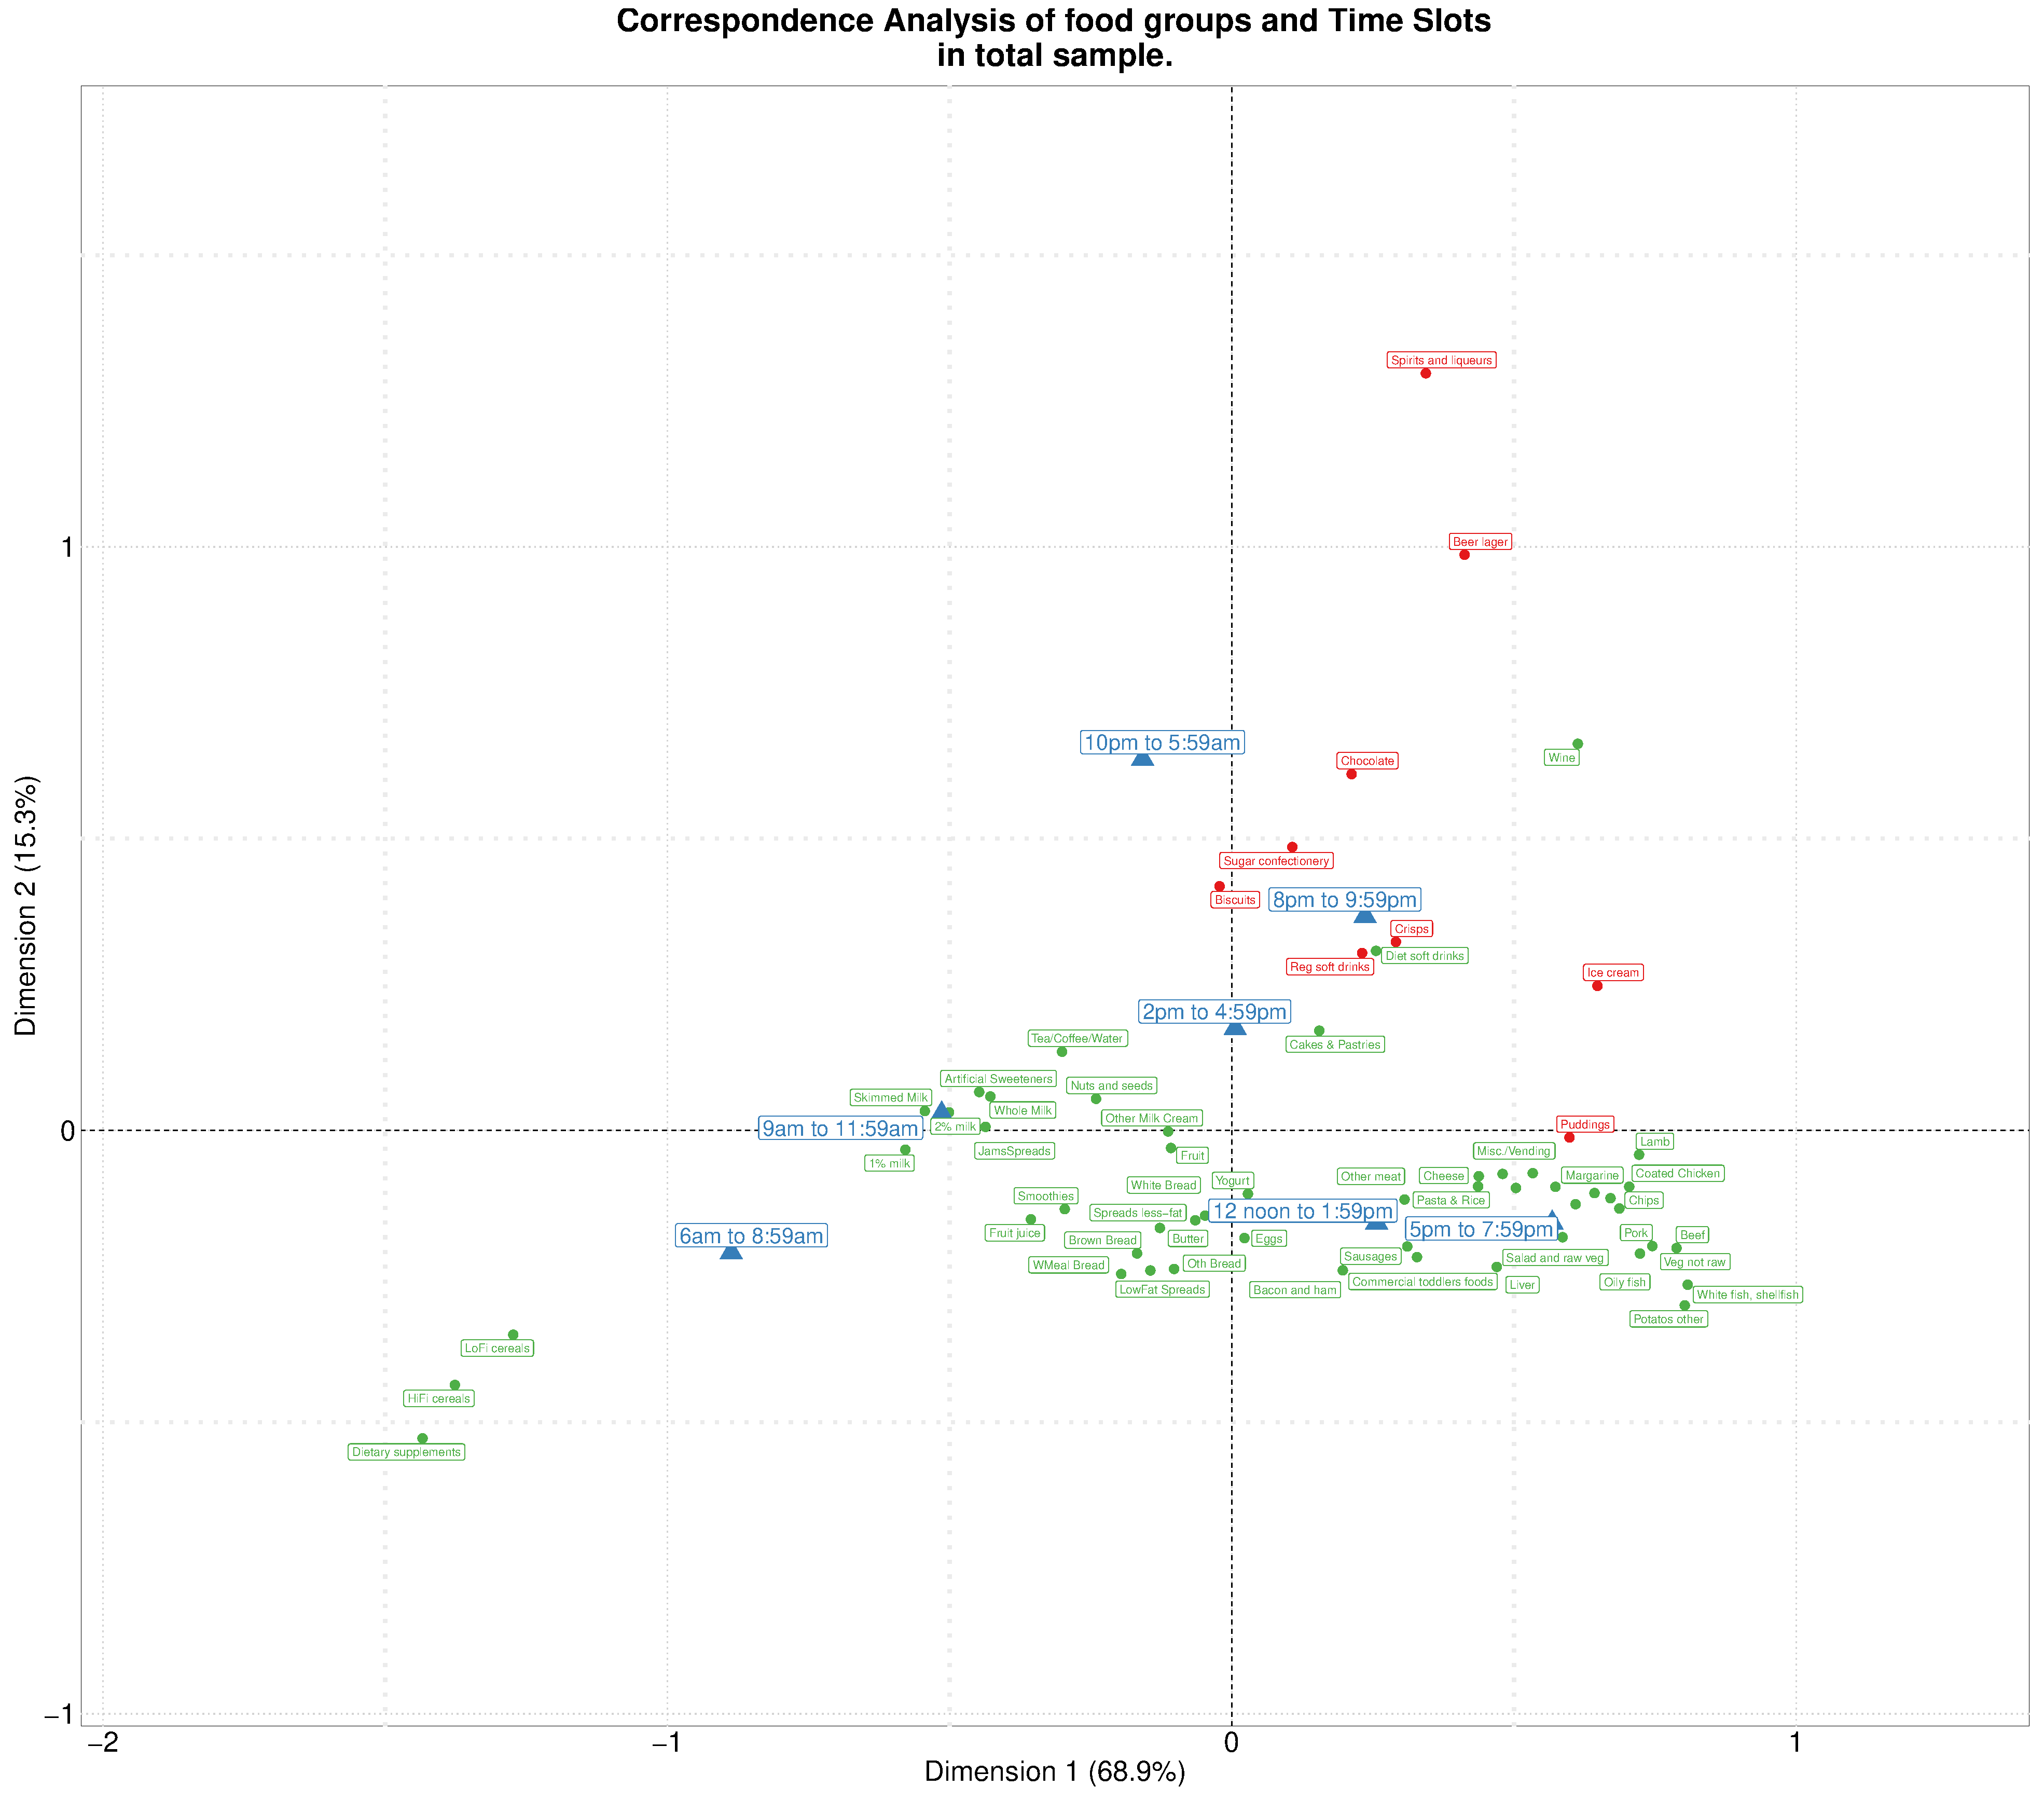
\includegraphics{Fig1.eps}
%	\caption{Biplot of food groups and eating time slots among total sample of NDNS RP.}
%	\label{fig1}
%\end{figure}


To visualize the potentially different associational patterns between food groups choice and time slots according to diabetes status, Figure 2-5 display the CA biplots in subsets of the data. Depending on different diabetes status, these biplots explained between 76.3\% and 84.1\% of the inertia in the data. Similarly to the biplot created from the total sample (Figure 1), later time in the day (8 pm and later) are shown in the upper side of each figure and suggested an association with the alcoholic beverages and highly processed or energy-dense food groups. Additionally, some food groups and time slots also flagged up associations potentially different by diabetes status. For example, puddings seemed to be closer to later time in the day among undiagnosed diabetics (Figure 4) while for diagnosed diabetic patients (Figure 3) they were closer to traditional dinner time (5 pm to 8 pm) or earlier in the day. Furthermore, sugar confectioneries/chocolates/biscuits/regular soft drinks appeared to be associated with later time in the day (8 pm or later) more strongly among undiagnosed diabetics (Figure 4) than the other participants.

Based on the findings suggested from Figure 1-5, we decided to focus on puddings, regular soft drinks, confectioneries, chocolates, spirits, beers, ice cream, biscuits, crisps as these foods either showed a particularly strong association with time of the day or a different pattern of association across different strata of the survey sample; hence, we tested the following null hypotheses using logistic regression models (adjusted for age, sex, and socio-economic levels) with GEE: that the odds of consuming each selected food at later time of the day (8 pm - 6 am) is the same compared to earlier in the day; and the associations of the above-mentioned food groups and time slots are the same among participants with different diabetes status (i.e. no interaction between the time of food intake and diabetes status). The results are summarized in Table 2. 

The listed food groups were found to have higher odds to be consumed between 8 pm and 6 am with higher odds compared to earlier time. The OR (99\% CIs) main effects of consuming these foods at evening/night were for puddings 1.38 (1.03, 1.86), for regular soft drinks 1.74 (1.47, 2.06), for sugar confectioneries 1.92 (1.38, 2.69), for chocolates 3.19 (2.69, 3.79), for spirits 11.13 (8.37, 14.80), for beers 7.19 (5.87, 8.82), for ice cream 2.38 (1.79, 3.15), for biscuits 1.91 (1.67, 2.16), for crisps 1.55 (1.27, 1.88) vs. earlier time. Opposite directions of the association for puddings were detected across diabetes status: the ORs (99\% CIs) of consuming puddings at night time (8 pm or later) compared to earlier time were 1.50 (1.10, 2.07),	0.89 (0.16, 4.87),	1.81 (0.41, 7.98), and	0.58 (0.14, 2.43) for healthy, prediabetic, undiagnosed diabetic, and diabetic participants, respectively. Furthermore, undiagnosed diabetic patients were found to have particularly high odds of consuming regular soft drinks (OR: 2.72; 99\% CI: 1.44, 5.14), and sugar confectioneries (OR: 13.07; 99\%CI: 4.59, 37.24) during night time periods compared to participants with other diabetes status. 




\section*{Discussion}


The present study described the potential relationships between food groups and time of their consumption in a representative sample from the NDNS RP. Many unhealthy foods emerged from CA were found to be more likely to be consumed after 8 pm. These included alcoholic/sweetened beverages, chocolates and other foods rich in added sugars and saturated fats such as biscuits and ice cream. Foods chosen in the evening/night time slots tend to be highly processed and easily accessible. Specifically, undiagnosed patients might be at a higher risk of worsening their condition as they were found to have higher odds to choose a number of less healthy foods after 8 pm (sugar confectioneries, regular soft drinks) than diabetics and non-diabetics. Those foods might need to be targeted when designing intervention to those who might be at risk of being diabetics. 

These findings are concerning considering previous research that have indicated that quality of macronutrient intake in the evening is likely to influence fasting glucose levels and glycaemic response to subsequent meals in the morning. \cite{Wolever1988} More recently, a randomized controlled trial indicated that consuming carbohydrates at dinner irrespective of glycaemic index raised postprandial glucose response to breakfast producing what is known as a second meal effect \cite{Haldar2020}. Similar observation have been made by Nitta and colleagues who observed that eating sweet snacks post-dinner worsened glycaemic excursions in the evening and at subsequent breakfast \cite{Nitta2019}. Added to this is evidence that suggests that the late-night dinners induce post-prandial hyperglycemia in patients with type 2 diabetes and that interventions at this eating occassions can result in a profound impact on post-prandial glycaemia. On the balance of this evidence, targeting and improving the timing and quality of foods in evening eating occasions provides a unique opportunity to design intervention to those who might be at risk of being diabetics. 


A compelling finding of our study is the observation that diabetes patients were found to be potentially controlling their choice of food groups such as avoiding puddings at night. However, higher odds of consuming alcoholic beverages and energy condensed foods such as chocolates and sugar confectioneries at night among individuals with diabetes suggests that their food choice might need further modifications. 

Assessing the relationships between food groups and timing of eating by diabetes status can be considered as a first step towards identifying specific public health targets for behavior change/intervention. This is important as most current public health strategies and dietary recommendations do not provide targeted advice that takes into considerations specific eating occasions while targeted advice is more likely to result in sustainable behavioural change. Our findings are consistent with previous evidence that has found that both sweetened and alcoholic beverages are responsible for large portion of energy consumption at night in other populations \cite{Hassen2018}. 


However, an important limitation in this study is the cross-sectional study design. The inability to assess the temporal relationship between timing of food intake and diabetes status means that a cause-effect relationship between time of unhealthy food intake and diabetes status cannot be established. Hence, further prospective studies are warranted to investigate the causal relationship between diabetes and both quality and timing of eating. Moreover, the current study assumes that mis-reporting occurred equally amongst all eating occasions. This limitation has been reported by previous literature as an important methodological limitation of chrononutrition \cite{FayetMoore2017}; in fact further investigation would be warranted to assess the effect of differential misreporting on epidemiological studies in chrono-nutrition in order to suggest possible corrections, e.g. for differential under-reporting at different times of the day (e.g. main meals vs. snack times). 


\section*{Conclusions}
In summary, our study indicates that foods consumed in the evening/night time tend to be highly processed, easily accessible, and rich in added sugar or saturated fat, whatever the diabetic status. . Individuals with undiagnosed diabetes are more likely to consume specific unhealthy foods at night. The survey cross-sectional nature warrants further investigations by longitudinal cohort studies to establish the causal relation between time of eating of unhealthy foods and diabetes.

%Text for this section\ldots
%\subsection*{Sub-heading for section}
%Text for this sub-heading\ldots
%\subsubsection*{Sub-sub heading for section}
%Text for this sub-sub-heading\ldots
%\paragraph*{Sub-sub-sub heading for section}
%Text for this sub-sub-sub-heading\ldots
%
%In this section we examine the growth rate of the mean of $Z_0$, $Z_1$ and $Z_2$. In
%addition, we examine a common modeling assumption and note the
%importance of considering the tails of the extinction time $T_x$ in
%studies of escape dynamics.
%We will first consider the expected resistant population at $vT_x$ for
%some $v>0$, (and temporarily assume $\alpha=0$)
%
%\[
%E \bigl[Z_1(vT_x) \bigr]=
%\int_0^{v\wedge
%1}Z_0(uT_x)
%\exp (\lambda_1)\,du .
%\]
%
%If we assume that sensitive cells follow a deterministic decay
%$Z_0(t)=xe^{\lambda_0 t}$ and approximate their extinction time as
%$T_x\approx-\frac{1}{\lambda_0}\log x$, then we can heuristically
%estimate the expected value as
%%
%\begin{equation}\label{eqexpmuts}
%\begin{aligned}[b]
%&      E\bigl[Z_1(vT_x)\bigr]\\
%&\quad      = \frac{\mu}{r}\log x
%\int_0^{v\wedge1}x^{1-u}x^{({\lambda_1}/{r})(v-u)}\,du .
%\end{aligned}
%\end{equation}
%
%Thus we observe that this expected value is finite for all $v>0$ (also see \cite{koon,xjon,marg,schn,koha,issnic}).





%\section*{Appendix}
%Text for this section\ldots

%%%%%%%%%%%%%%%%%%%%%%%%%%%%%%%%%%%%%%%%%%%%%%
%%                                          %%
%% Backmatter begins here                   %%
%%                                          %%
%%%%%%%%%%%%%%%%%%%%%%%%%%%%%%%%%%%%%%%%%%%%%%

\begin{backmatter}

\section*{Acknowledgements}%% if any
%Text for this section\ldots
We thank the NDNS team at former MRC Elsie Widdowson Laboratory in Cambridge and NatCen Social Research in London for providing information about data collection and coding. 

\section*{Funding}%% if any
This work was supported by Grants-in-Aid for Young Scientists (grant number 19K20199 to C.W.) from the Japan Society for the Promotion of Science (JSPS).

%\sec%tion*{Abbreviations}%% if any
%to be updated \ldots

\section*{Availability of data and materials}%% if any
Original data used in this study can be accessed upon request to the UK Data Service (https://www.ukdataservice.ac.uk) for academic usage (Study Number: 6533).

\section*{Ethics approval and consent to participate}%% if any
The NDNS RP, funded by Public Health England and the UK Food Standards Agency, is registered with the ISRTCN registry under study ID ISRCTN17261407 and received ethical approval from the Oxfordshire Research Ethics Committee. 

\section*{Competing interests}
The authors declare that they have no competing interests.

\section*{Consent for publication}
Not applicable.

\section*{Authors' contributions}
CW, SA, and LP: designed research and had primary responsibility for final content; CW and LP performed statistical analysis; and all authors: wrote the manuscript, read and approved the final manuscript.

%\section*{Authors' information}%% if any
%Text for this section\ldots

%%%%%%%%%%%%%%%%%%%%%%%%%%%%%%%%%%%%%%%%%%%%%%%%%%%%%%%%%%%%%
%%                  The Bibliography                       %%
%%                                                         %%
%%  Bmc_mathpys.bst  will be used to                       %%
%%  create a .BBL file for submission.                     %%
%%  After submission of the .TEX file,                     %%
%%  you will be prompted to submit your .BBL file.         %%
%%                                                         %%
%%                                                         %%
%%  Note that the displayed Bibliography will not          %%
%%  necessarily be rendered by Latex exactly as specified  %%
%%  in the online Instructions for Authors.                %%
%%                                                         %%
%%%%%%%%%%%%%%%%%%%%%%%%%%%%%%%%%%%%%%%%%%%%%%%%%%%%%%%%%%%%%

% if your bibliography is in bibtex format, use those commands:
\bibliographystyle{bmc-mathphys} % Style BST file (bmc-mathphys, vancouver, spbasic).
\bibliography{bmc_article}      % Bibliography file (usually '*.bib' )
% for author-year bibliography (bmc-mathphys or spbasic)
% a) write to bib file (bmc-mathphys only)
% @settings{label, options="nameyear"}
% b) uncomment next line
%\nocite{label}

% or include bibliography directly:
% \begin{thebibliography}
% \bibitem{b1}
% \end{thebibliography}

%%%%%%%%%%%%%%%%%%%%%%%%%%%%%%%%%%%
%%                               %%
%% Figures                       %%
%%                               %%
%% NB: this is for captions and  %%
%% Titles. All graphics must be  %%
%% submitted separately and NOT  %%
%% included in the Tex document  %%
%%                               %%
%%%%%%%%%%%%%%%%%%%%%%%%%%%%%%%%%%%

%%
%% Do not use \listoffigures as most will included as separate files

\section*{Figures}
  \begin{figure}[h!]
%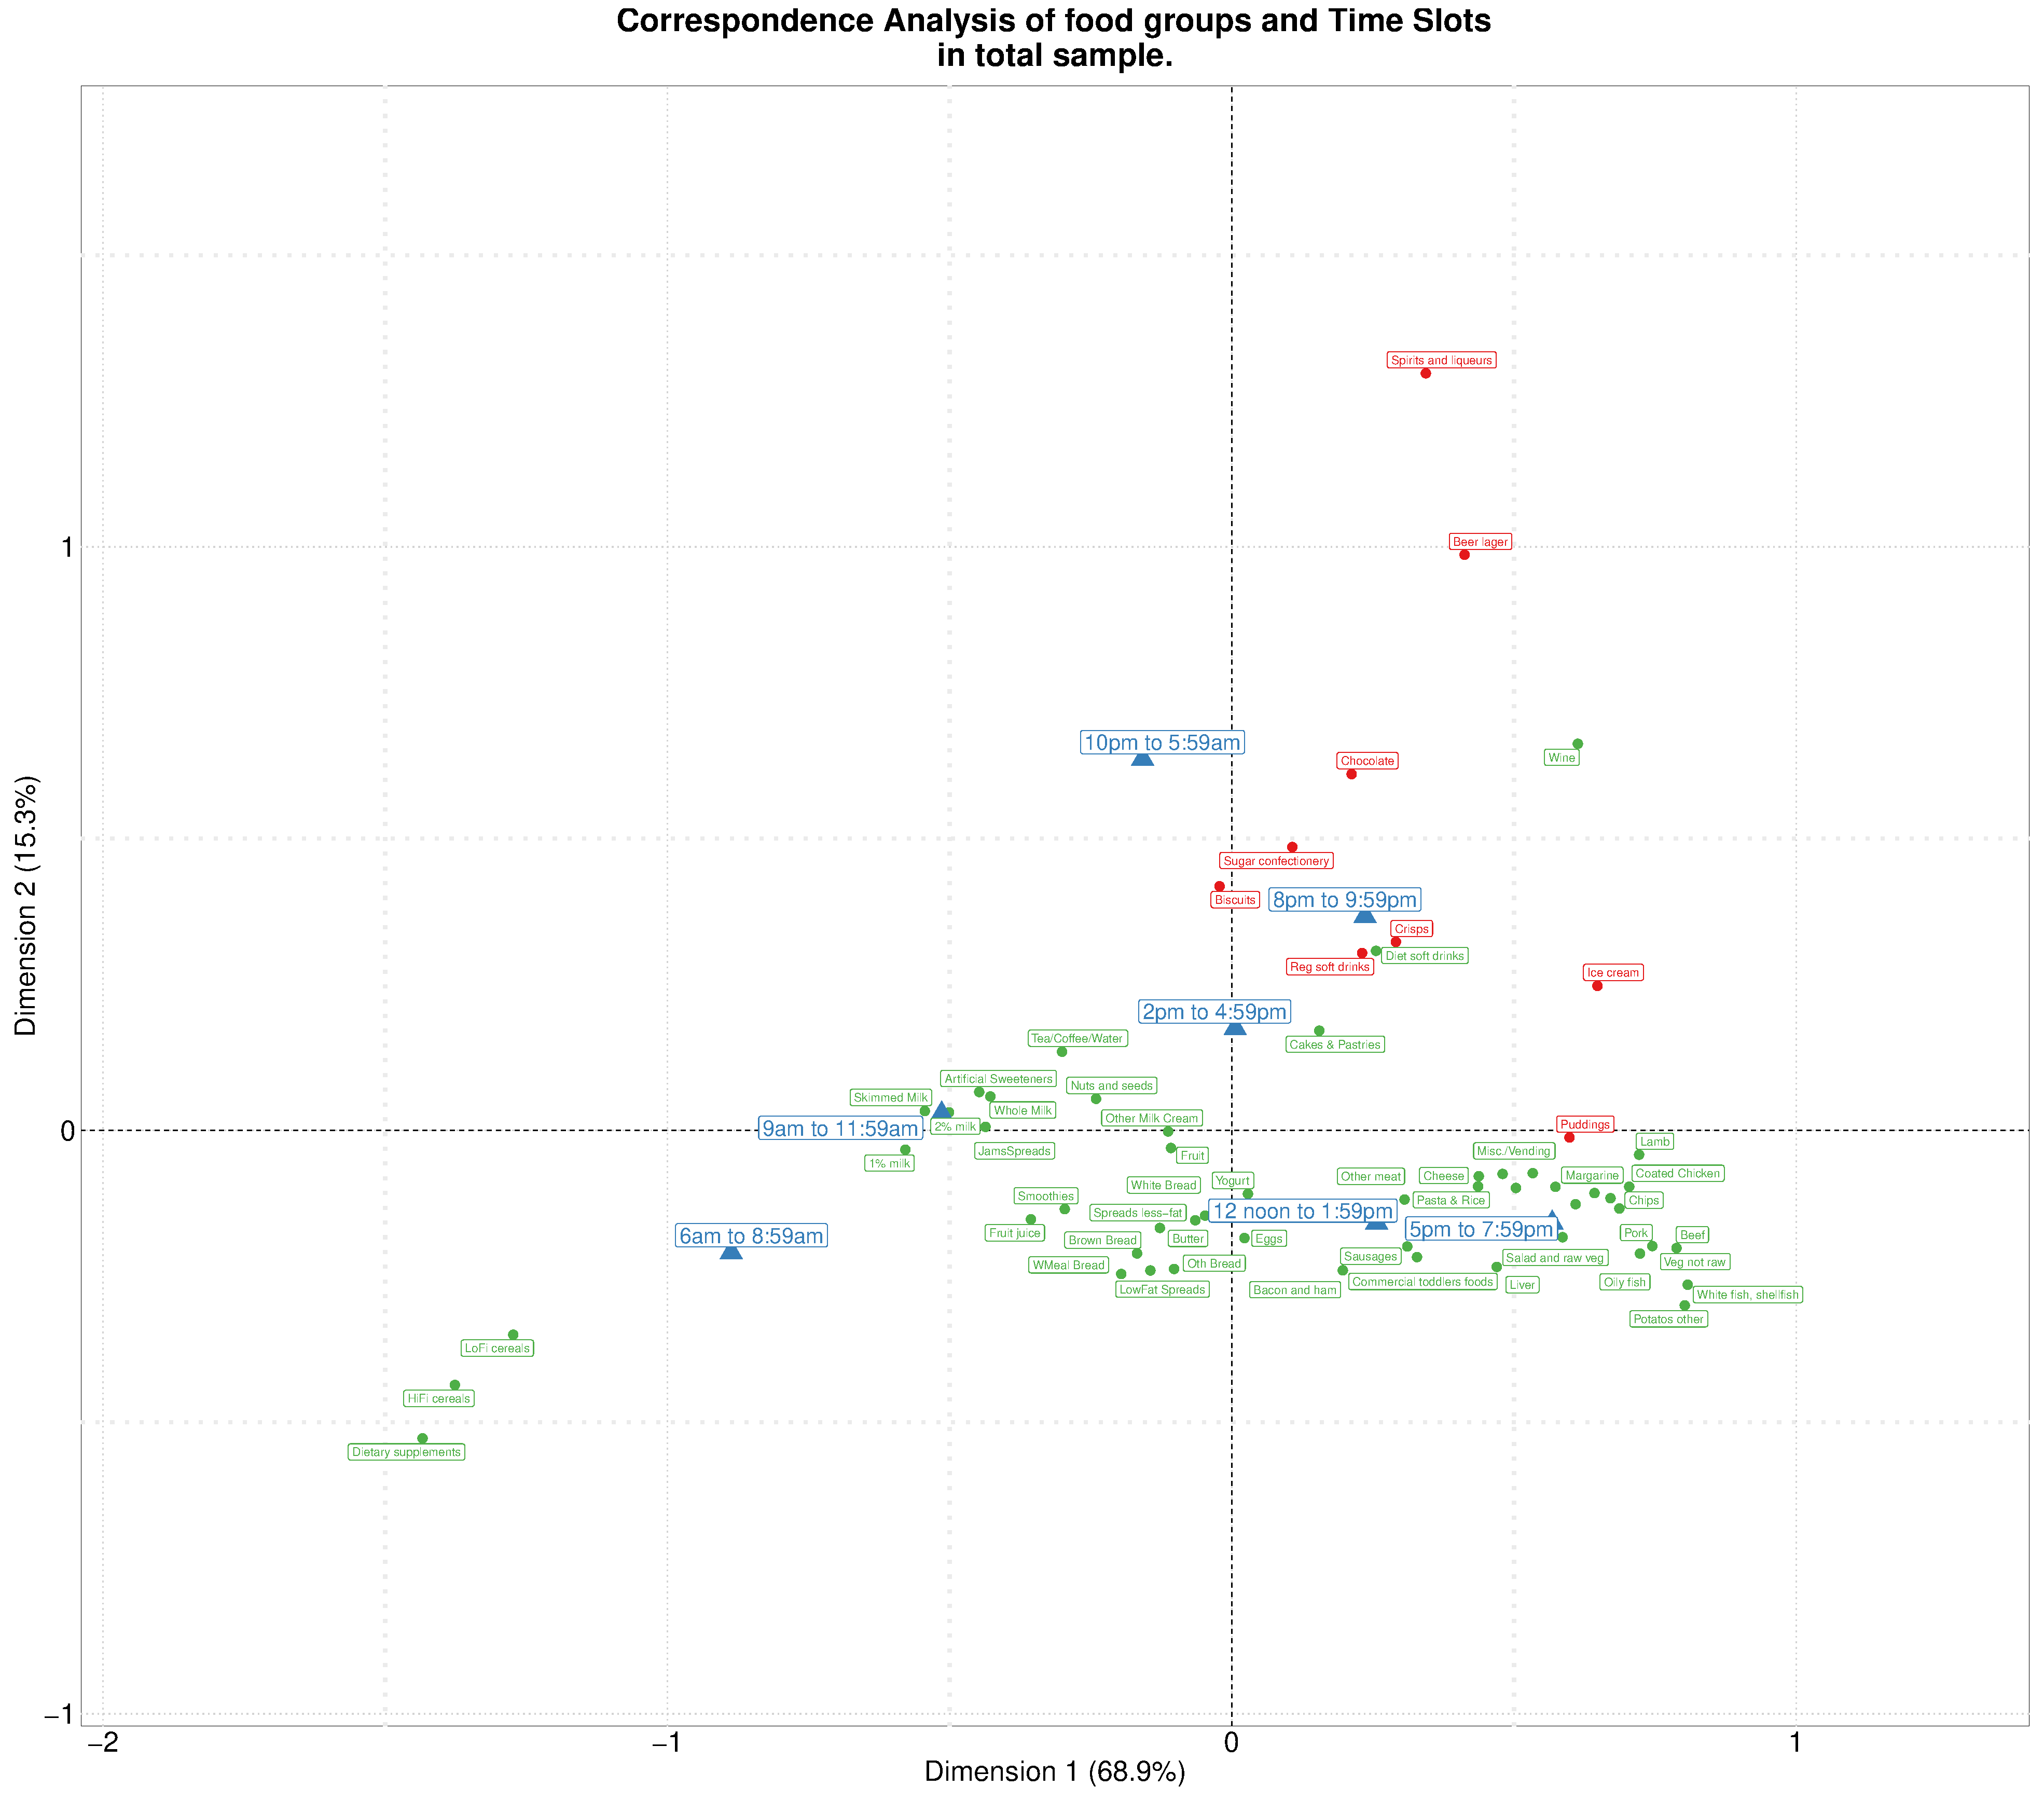
\includegraphics{Fig1.eps}
  \caption{Biplot of food groups and eating time slots among total sample of NDNS RP.}
\end{figure}

\begin{figure}[h!]
  \caption{Biplot of food groups and eating time slots among non-diabetics.}
\end{figure}

\begin{figure}[h!]
	\caption{Biplot of food groups and eating time slots among diabetics.}
\end{figure}

\begin{figure}[h!]
	\caption{Biplot of food groups and eating time slots among undiagnosed diabetics.}
\end{figure}


\begin{figure}[h!]
	\caption{Biplot of food groups and eating time slots among pre-diabetics.}
\end{figure}


%%%%%%%%%%%%%%%%%%%%%%%%%%%%%%%%%%%
%%                               %%
%% Tables                        %%
%%                               %%
%%%%%%%%%%%%%%%%%%%%%%%%%%%%%%%%%%%

%% Use of \listoftables is discouraged.
%%
\section*{Tables}

\begin{table}[h!]
	\caption{The numbers of food recordings contributed to the total calories consumed by adults in the UK adults. (NDNS RP 2008-2017).}
	\begin{tabular}{lccccc}
		Food group names                                    & n     & Calories   & Relative Prop & Cal Prop & Cal Cum Prop \\\hline
		Pasta \& Rice and other cereals                     & 18353 & 3512069.99 & 2.45\%        & 7.36\%   & 7.36\%       \\
		White Bread                                         & 18434 & 3245641.19 & 2.46\%        & 6.80\%   & 14.17\%      \\
		Chips, fried and roast potatoes and potato products & 6749  & 1884058.68 & 0.90\%        & 3.95\%   & 18.12\%      \\
		Cakes, buns, sweet pastries, fruit pies             & 7806  & 1710594.27 & 1.04\%        & 3.59\%   & 21.70\%      \\
		Vegetable (not raw)                                 & 51317 & 1665474.02 & 6.85\%        & 3.49\%   & 25.19\%      \\
		Biscuits                                            & 13200 & 1662598.06 & 1.76\%        & 3.49\%   & 28.68\%      \\
		Fruit                                               & 33903 & 1641675.02 & 4.53\%        & 3.44\%   & 32.12\%      \\
		Miscellaneous unclassified foods                    & 48597 & 1639024.81 & 6.49\%        & 3.44\%   & 35.56\%      \\
		Chicken/turkey                                      & 8863  & 1617820.30 & 1.18\%        & 3.39\%   & 38.95\%      \\
		Cheese                                              & 10983 & 1492015.32 & 1.47\%        & 3.13\%   & 42.07\%      \\
		Beer lager                                          & 8199  & 1484001.20 & 1.09\%        & 3.11\%   & 45.19\%      \\
		Semi-skimmed milk                                   & 57611 & 1302649.72 & 7.69\%        & 2.73\%   & 47.92\%      \\
		Potatos other (in salads and dishes)                & 10113 & 1291447.61 & 1.35\%        & 2.71\%   & 50.62\%      \\
		Fat spreads                                         & 37960 & 1215278.60 & 5.07\%        & 2.55\%   & 53.17\%      \\
		Beef                                                & 4987  & 1124560.42 & 0.67\%        & 2.36\%   & 55.53\%      \\
		High fiber breakfast cereals                        & 8215  & 1072813.73 & 1.10\%        & 2.25\%   & 57.78\%      \\
		Whole meal bread                                    & 7193  & 1070695.89 & 0.96\%        & 2.24\%   & 60.02\%      \\
		Chocolate                                           & 6495  & 1046112.65 & 0.87\%        & 2.19\%   & 62.22\%      \\
		Wine                                                & 6967  & 1027792.96 & 0.93\%        & 2.15\%   & 64.37\%      \\
		Brown, granary and wheatgerm bread                  & 6183  & 1009074.95 & 0.83\%        & 2.12\%   & 66.48\%      \\
		Butter                                              & 10203 & 965901.11  & 1.36\%        & 2.02\%   & 68.51\%      \\
		Eggs                                                & 7554  & 964769.19  & 1.01\%        & 2.02\%   & 70.53\%      \\
		Soft drinks not diet                                & 11387 & 940516.516 & 1.52\%        & 1.97\%   & 72.50\%      \\
		Reduced fat spreads                                 & 12620 & 848834.89  & 1.68\%        & 1.78\%   & 74.28\%      \\
		Crisps and savoury snacks                           & 5664  & 835671.58  & 0.76\%        & 1.75\%   & 76.04\%      \\
		Sausages                                            & 3025  & 775004.13  & 0.40\%        & 1.62\%   & 77.66\%      \\
		Meat pastries                                       & 1979  & 744639.89  & 0.26\%        & 1.56\%   & 79.22\%      \\
		Bacon and ham                                       & 8467  & 738727.49  & 1.13\%        & 1.55\%   & 80.77\%      \\
		Yogurt                                              & 6776  & 665484.55  & 0.90\%        & 1.40\%   & 82.16\%      \\
		Low-fiber breakfast cereals                         & 4303  & 560296.32  & 0.57\%        & 1.17\%   & 83.34\%      \\
		Nuts and seeds                                      & 6259  & 559873.88  & 0.84\%        & 1.17\%   & 84.51\%      \\
		Oily fish                                           & 2610  & 550425.36  & 0.35\%        & 1.15\%   & 85.67\%      \\
		Whole Milk                                          & 13628 & 530449.07  & 1.82\%        & 1.11\%   & 86.78\%      \\
		White fish, shellfish                               & 1597  & 498928.82  & 0.21\%        & 1.05\%   & 87.82\%      \\
		Puddings                                            & 2291  & 459784.62  & 0.31\%        & 0.96\%   & 88.79\%      \\
		Other Milk Cream                                    & 6605  & 434239.37  & 0.88\%        & 0.91\%   & 89.70\%      \\
		Pork                                                & 1832  & 420503.76  & 0.24\%        & 0.88\%   & 90.58\%     \\\hline
		\multicolumn{6}{l}{NDNS RP: National Diet and Nutrition Survey. }
	\end{tabular}
\end{table}


\begin{table}[h!]
	\caption{Odds ratio (99\% confidence intervals) for food groups eaten at night (8 pm - 6 am) vs. earlier time in the day, among total and according to different diabetes status, NDNS RP 2008-2017.}
	\begin{tabular}{llllll}
		Selected food groups & Overall             & Healthy             & Pre-diabetics      & Undiagnosed diabetes & Diabetes            \\\hline
		Pudding              & 1.38 (1.03, 1.86)   & 1.50 (1.10, 2.07)   & 0.89 (0.16, 4.87)  & 1.81 (0.41, 7.98)    & 0.58 (0.14, 2.43)   \\
		Regular soft drink   & 1.74 (1.47, 2.06)   & 1.72 (1.43, 2.06)   & 1.87 (0.97, 3.57)  & 2.72 (1.44, 5.14)    & 1.38 (0.65, 2.96)   \\
		Sugar Confectionery  & 1.92 (1.38, 2.69)   & 1.63 (1.14, 2.32)   & 2.10 (0.52, 8.46)  & 13.07 (4.59, 37.24)  & 5.10 (2.15, 12.09)  \\
		Chocolate            & 3.19 (2.69. 3.79)   & 3.10 (2.57, 3.73)   & 4.07 (2.58, 3.73)  & 2.52 (0.95, 6.66)    & 5.13 (2.55, 10.30)  \\
		Spirit               & 11.13 (8.37, 14.80) & 10.86 (8.01, 14.73) & 8.48 (2.26, 31.79) & 7.51 (1.99, 5.21)    & 36.8 (7.36, 183.66) \\
		Beer                 & 7.19 (5.87, 8.82)   & 7.49 (6.02, 9.34)   & 4.05 (2.00, 8.20)  & 7.87 (3.51, 17.63)   & 6.32 (2.29, 17.47)  \\
		Ice Cream            & 2.38 (1.79, 3.15)   & 2.45 (1.82, 3.31)   & 3.32 (0.75, 14.62) & 0.98 (0.14, 7.00)    & 1.65 (0.54, 5.07)   \\
		Biscuit              & 1.91 (1.67, 2.16)   & 1.78 (1.55, 2.03)   & 3.51 (2.16, 5.71)  & 2.75 (1.35, 5.59)    & 2.44 (1.54, 3.88)   \\
		Crisp                & 1.55 (1.27, 1.88)   & 1.56 (1.27, 1.92)   & 1.95 (0.79, 4.78)  & 1.37 (0.37, 5.12)    & 1.16 (0.49, 2.75)   \\\hline
		\multicolumn{6}{l}{Logistic regression models with GEE were adjusted for age, sex, and social-economic levels.}  \\
				\multicolumn{6}{l}{NDNS RP: National Diet and Nutrition Survey. }             
	\end{tabular}
\end{table}





%%%%%%%%%%%%%%%%%%%%%%%%%%%%%%%%%%%
%%                               %%
%% Additional Files              %%
%%                               %%
%%%%%%%%%%%%%%%%%%%%%%%%%%%%%%%%%%%

%\section*{Additional Files}
%  \subsection*{Additional file 1 --- Sample additional file title}
%    Additional file descriptions text (including details of how to
%    view the file, if it is in a non-standard format or the file extension).  This might
%    refer to a multi-page table or a figure.

 % \subsection*{Additional file 2 --- Sample additional file title}
 %   Additional file descriptions text.

\end{backmatter}
\end{document}